The most common types of recommender systems can be split into collaborative filtering and content based. They can be further split into model-based, and memory-based.

\subsection{Content Based}
Content based recommendations require several features related to an item instead of historic user-item interactions. In the case of movie recommendations, these could be year, actors, genres, producers, writers, etc.
This method relies on calculating the similarity between items using features such as the ones previously stated.
The general idea is that if a user likes a given item he will also like items similar to it. One way of achieving this is by calculating term frequency (TF) and inverse document frequency (IDF) of the items. Then using the vector space model and a choice of similarity metrics such as cosine or pearson, we can compare different items (\citet{contentrs}).
Another way of achieving this is to represent different content items as dense vectors that can be easily fed into a neural network architecture.

\subsection{Collaborative Filtering}
Collaborative filtering (CF) algorithms aim to recommend items to a user by combining the item interactions of a given user with item interactions of all other users. CF can be split into two categories. User-based where the aim is to measure the similarity of a given user and all other users (\citet{usercf}). Item-based where we aim to measure the similarity between the items a given user has interacted with and other items (\citet{itemcf}).
The most widely used method of achieving this is through factorization of the very sparse user-item interaction matrix.

\subsection{Matrix Factorization}
The idea behind matrix factorization (MF) is to decompose the matrix R containing user-item interactions, into the product of two lower dimensional matrices P of size \(n X k\) and Q of size \(k X m\). Matrix P is the user matrix where n is the number of users, k the number of latent factors and \(p_u\) is the latent vector of user u. The other matrix is the movie matrix with m number of movies, the same k latent factors and \(q_i\) is the latent vector of item i. The predicted rating \(\hat{y}_{ui}\) can then be calculated by taking the dot product of those two vectors (\citet{MF_Techniques}).

\begin{equation}
    \hat{y}_{ui} = f(u,i|P_{u}Q_{i}) = P_{u}^{T}Q_{i} = \sum_{K=0}^{k}P_{uk}Q_{ik}
\end{equation}

Singular value decomposition (SVD) and non-negative matrix factorization (NMF) are two techniques successfully applied in literature to achieve the decomposition (\citet{svd}).

The resulting matrices are dense and have much lower dimension than the initial matrix R. By choosing a different number of latent factors we can include more or less abstract information. MF poses the recommendation problem as a regression optimization one. Two common optimization metrics used for this are root mean squared error (RMSE) and mean absolute error (MAE). The RMSE and MAE can be calculated as follows given that, \(e_i\) is the difference between the actual and predicted value of rating i. 
\begin{equation}
    RMSE = \sqrt{\frac{1}{n}\sum_{i=1}^{n}{e^2_i}}
\end{equation}
\begin{equation}
    MAE = \frac{1}{n}\sum_{i=1}^{n}{\mid e_i\mid}
\end{equation}

Stochastic gradient descent (SGD) and alternating least square (ALS) are two optimization algorithm generally employed to learn a good approximation for the matrices. ALS is more often used for implicit dataset because its more efficient than SGD on such data. The algorithm is succinctly described below.
\begin{itemize}
    \item 1. Set item factor matrix constant and adjust user factor matrix.
    \item 2. Set user factor matrix constant and adjust item factor matrix.
    \item Repeat until convergence.
\end{itemize}

\subsection{Neural Networks \& Deep Learning}
Neural networks are universal approximators, typically organized in layers of neurons connected through weights and put through an activation function. The number of layers and neurons at each layer also called the depth and width of the network are variable and many different configurations seem to work in practice. The simplest neural network is made up of 3 layers, input, hidden and output.

\begin{figure}[h!]
    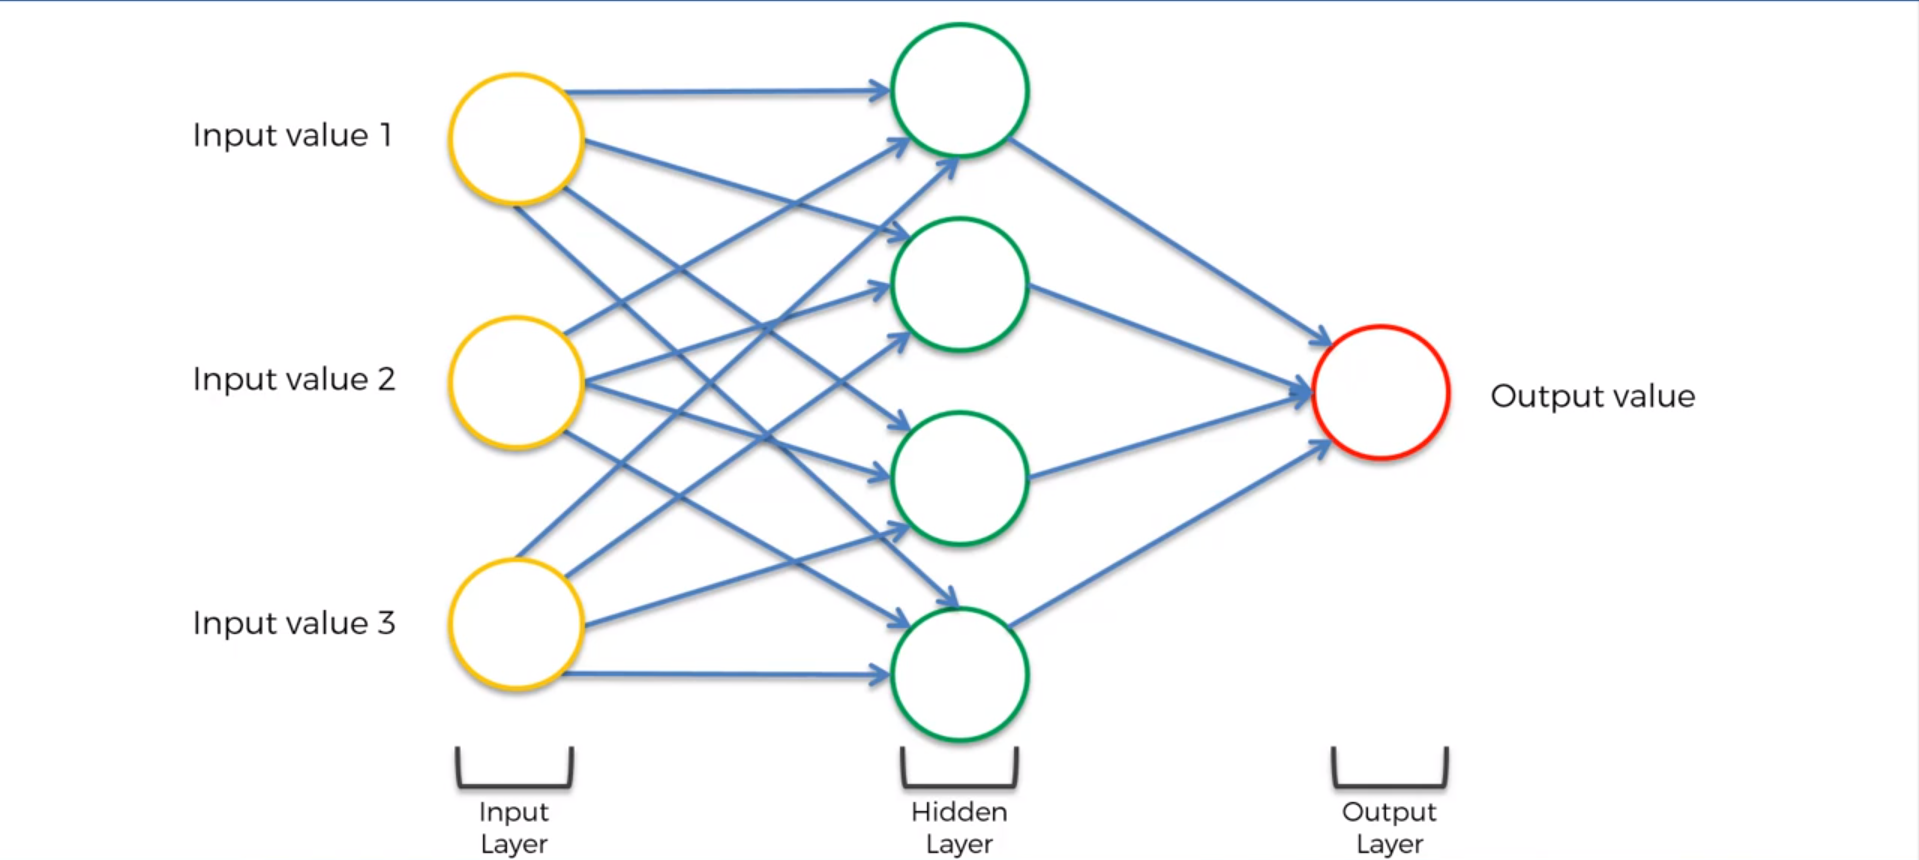
\includegraphics[scale=0.2]{nn-3-layers}
    \caption{3 Layer Neural Network}
\end{figure}

They can be used for both supervised and unsupervised learning and can be applied to classification and regression problems just as effectively. Deep neural networks (DNN) are NN of more than 3 layers, although in practice and state of the art implementations these are many layers deep and very wide as well. The main benefit of using NNs algorithms is that they don't require manual feature engineering.
A big disadvantage is the lack of interpretability for the predictions, due to this NN are generally viewed as black boxes. This means that we are not aware of the `why` and `how` did the network product a certain output given some inputs. This could be especially detrimental in the context of recommendation systems because the users might wish to know the reasons behind their recommendations. Other memory and similarity based methods provide much more transparency in this regard.

At the core of DNNs success in modeling complex function is the back propagation algorithm. The back-propagation algorithm allows the network to learn by propagating the loss, calculated at the output layer, backwards to update the weights at each layer (\citet{backpropagation}). It uses the chain and product calculus rules to compute partial derivatives of the cost function for each node in the network. 

Different classes of NN have emerged in literature including convolutional networks (\citet{cnn}), autoencoders (\citet{autoencoders}), recurrent networks (\citet{rnn}), generative adversarial networks (\citet{gan}), besides of simple fully connected multilayer perceptrons.

\subsection{Related Work}
\citet{HybridAutoencoders} propose a hybrid recommender system based on auto-encoders. They use a loss function adapted to data with missing values. They also describe models that incorporate side information and find out these models deal better with the cold-start problem.
\citet{NeuralCF} propose a neural collaborative filtering system trained using implicit data. They design a novel ensemble framework that joins together generalized matrix factorization (GMF) and multilayer perceptron (MLP). The inputs to the network are user and item ids which are embedded into dense low dimensional vectors. The embeddings are shared by both GMF and MLP. GMF is supposed to mimic MF techniques and works by taking the dot product of the item and user embeddings. The user and item embeddings are concatenated before being fed into MLP. 
They train the network using Adam optimizer and ReLU activation functions in the MLP. Their results show that more layers in the MLP leads to better performance while keeping the number of factors constant. Furthermore, they compare the ensembles effectiveness with similarity and model based state of the art models and report 4\% improvement in hit ratio.
